%%%%%%%%%%%%%%%%%%%%%%%%%%%%%%%%%%%%%%%%%%%%%%%%%%%%%%%%%%%%%%%%%%%%%%%%%%%%%%%%%%%%%%%%%%%%%%%%%%%%%%%%%%%%%%%%%%%%%%%%%
\subsection{Weighted Paper-Ego-Network Construction}
%%%%%%%%%%%%%%%%%%%%%%%%%%%%%%%%%%%%%%%%%%%%%%%%%%%%%%%%%%%%%%%%%%%%%%%%%%%%%%%%%%%%%%%%%%%%%%%%%%%%%%%%%%%%%%%%%%%%%%%%%

%%%%%%%%%%%%%%%%%%%%%%%%%%%%%%%%%%%%%%%%%%%%%%%%%%%%%%%%%%%%%%%%%%%%%%%%%%%%%%%%%%%%%%%%%%%%%%%%%%%%%%%%%%%%%%%%%%%%%%%%%
\begin{frame}
\frametitle{Heterogeneous Information Network (HIN)}
\begin{columns}
\column{0.5\textwidth}

\begin{itemize}
    \item HINs are complex structures
    \item Complex structures lead to complex algorithms
    \item How to simply this HIN without removing relevant information?
\end{itemize}

\column{0.5\textwidth}
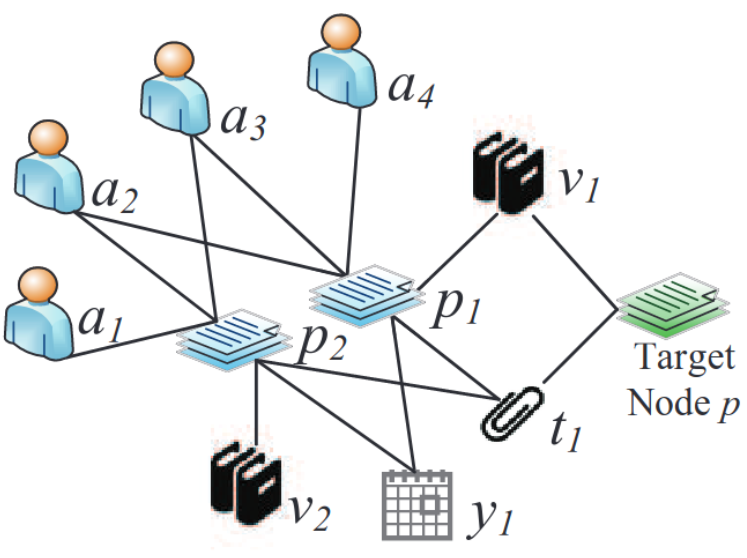
\includegraphics[width=1\linewidth]{img/hin}


\end{columns}
\end{frame}
%%%%%%%%%%%%%%%%%%%%%%%%%%%%%%%%%%%%%%%%%%%%%%%%%%%%%%%%%%%%%%%%%%%%%%%%%%%%%%%%%%%%%%%%%%%%%%%%%%%%%%%%%%%%%%%%%%%%%%%%
\begin{frame}
\frametitle{Weighted Paper-Ego-Network}
\begin{columns}
\column{0.5\textwidth}

\begin{itemize}
    \item Extraction of a task-guided embedding to learn the low-dimensional representation of network
    \item Creation of a simpler weighted graph
\end{itemize}

\column{0.5\textwidth}
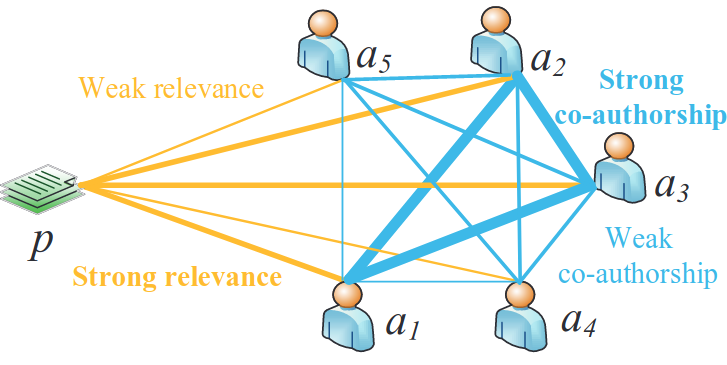
\includegraphics[width=1\linewidth]{img/paper-ego}


\end{columns}
\end{frame}
%%%%%%%%%%%%%%%%%%%%%%%%%%%%%%%%%%%%%%%%%%%%%%%%%%%%%%%%%%%%%%%%%%%%%%%%%%%%%%%%%%%%%%%%%%%%%%%%%%%%%%%%%%%%%%%%%%%%%%%%%
\subsection{Optimal Quasi-Clique with Constraint Extraction}
%%%%%%%%%%%%%%%%%%%%%%%%%%%%%%%%%%%%%%%%%%%%%%%%%%%%%%%%%%%%%%%%%%%%%%%%%%%%%%%%%%%%%%%%%%%%%%%%%%%%%%%%%%%%%%%%%%%%%%%%%

%%%%%%%%%%%%%%%%%%%%%%%%%%%%%%%%%%%%%%%%%%%%%%%%%%%%%%%%%%%%%%%%%%%%%%%%%%%%%%%%%%%%%%%%%%%%%%%%%%%%%%%%%%%%%%%%%%%%%%%%%
\begin{frame}
\frametitle{Optimal Author Subset}
\begin{columns}
\column{0.5\textwidth}

\begin{itemize}
    \item To find an optimal author subset that is related to the anonymous paper is a NP-hard problem
    \item Discovering the largest clique is inapproachable and the clique concept is in practice too strict to miss a single edge in an otherwise dense subgraph
    \item Quasi-clique has been significantly used to discover dense subgraphs
\end{itemize}

\column{0.5\textwidth}
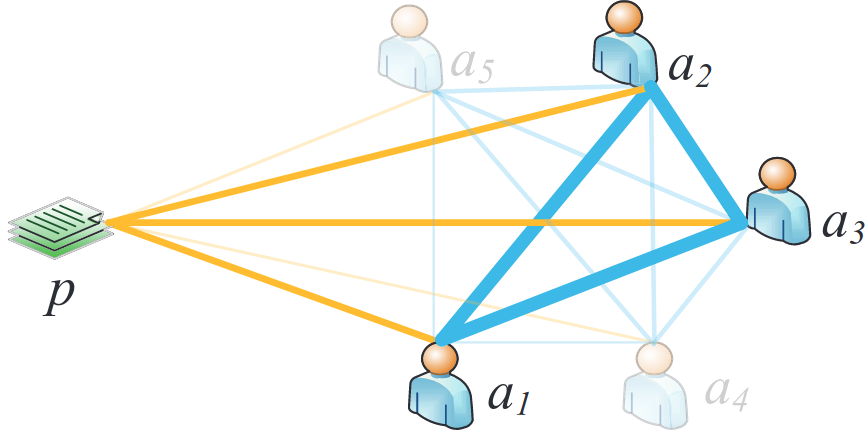
\includegraphics[width=1\linewidth]{img/paper-ego-solved}


\end{columns}
\end{frame}
%%%%%%%%%%%%%%%%%%%%%%%%%%%%%%%%%%%%%%%%%%%%%%%%%%%%%%%%%%%%%%%%%%%%%%%%%%%%%%%%%%%%%%%%%%%%%%%%%%%%%%%%%%%%%%%%%%%%%%%%%
\begin{frame}
\frametitle{Algorithm description}
\begin{columns}
\column{0.5\textwidth}

\begin{itemize}
    \item Optimization problem
    \item Local search algorithm
\end{itemize}

\column{0.5\textwidth}
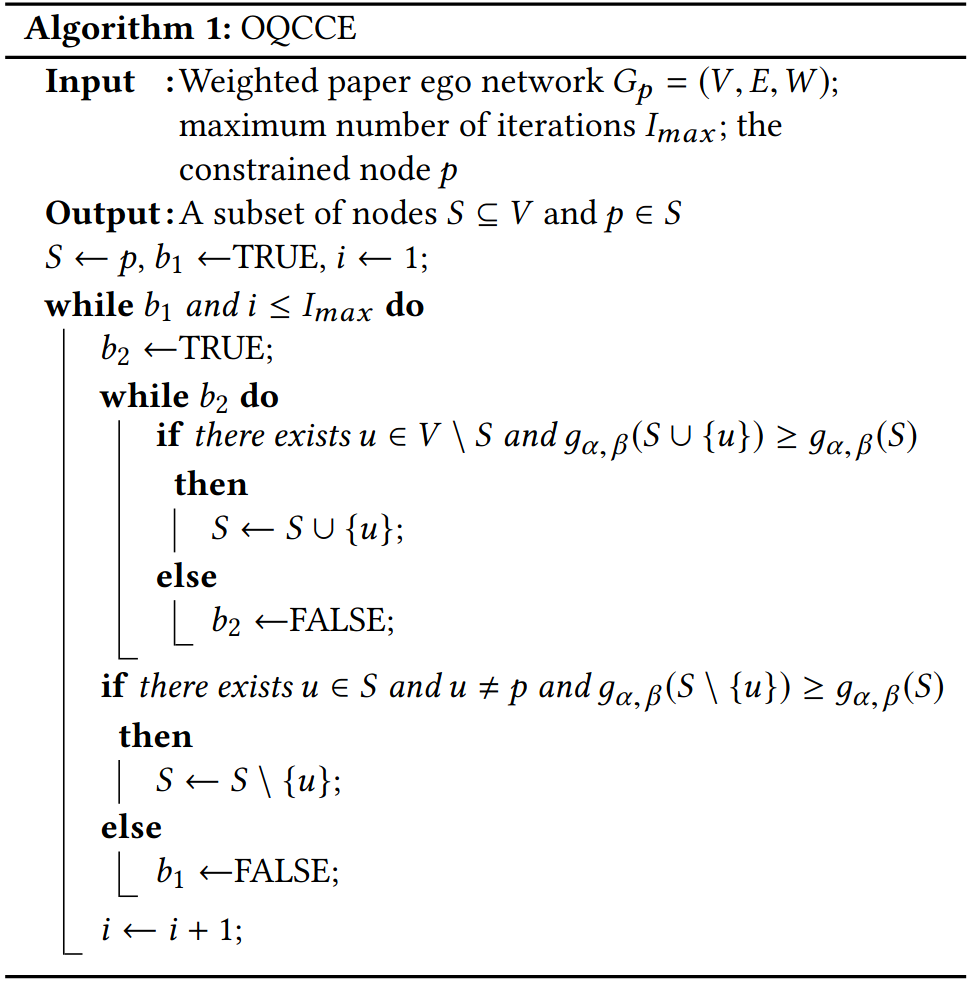
\includegraphics[width=1\linewidth]{img/algorithm}


\end{columns}
\end{frame}
%%%%%%%%%%%%%%%%%%%%%%%%%%%%%%%%%%%%%%%%%%%%%%%%%%%%%%%%%%%%%%%%%%%%%%%%%%%%%%%%%%%%%%%%%%%%%%%%%%%%%%%%%%%%%%%%%%%%%%%%